Na rys.~\ref{fig:2} przedstawiono wyniki
eksperymentu~\ref{subsec:rhodobacter}.
W 10 dniu eksperymentu widoczny jest istotny
statystycznie spadek \acrshort{od}\textsubscript{600}
w próbkach o $c_{\acrshort{ww}} = 80$ \% względem próbek
o niższych stężeniach.
Oznacza to hamowanie wzrostu \textit{R. spheroides}
przy stężeniach \acrshort{ww} 80 \%.
Z~tego względu w kolejnych eksperymentach kultywowano
\textit{R. spheroides} na \acrshort{m27} + 50 \% \acrshort{ww}\@.
Rys.~\ref{fig:3} przedstawia wyniki
eksperymentu~\ref{subsec:mlra}.
(\ldots)
Na rys.~\ref{fig:4} przedstawiono wyniki pomiarów
napięcia w eksperymencie~\ref{subsec:volt}.
Z wykresu wynika, że największe napięcia generowane
są w przypadku hodowli \textit{R. spheroides}
o \acrshort{od}\textsubscript{600} w zakresie od 0.200 do 0.535,
przy czym hodowle gęstsze, o~\acrshort{od}\textsubscript{600} bliskim
0.500 wykazują spadki napięcia po dłuższym czasie.

\begin{figure}[h!]
    \centering
    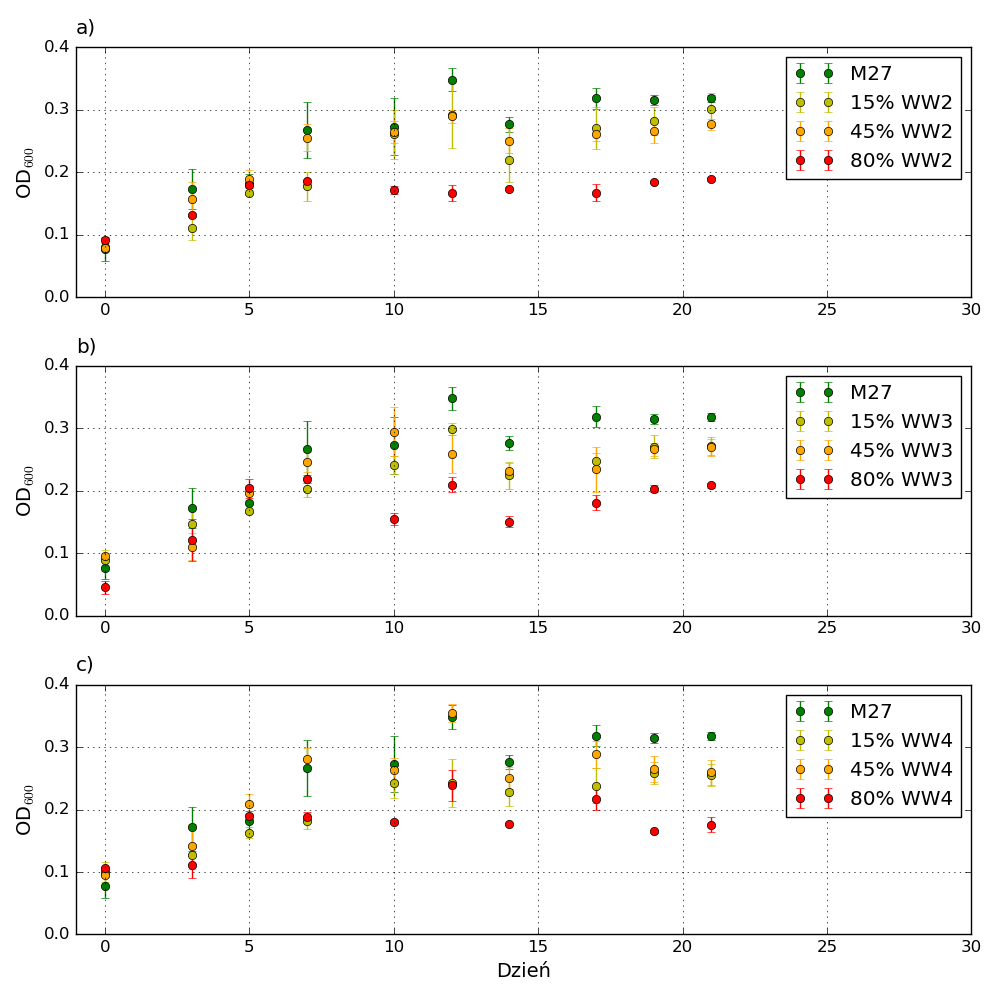
\includegraphics[width=13cm]{figures/ww}
    \caption{
        Zmiany \acrshort{od}\textsubscript{600} hodowli \textit{R. spheroides} w czasie w \acrshort{m27}:
        a)~zawierającym \acrshort{ww}2 w~stężeniach 15 \%, 45 \% i 80 \%;
        b)~zawierającym \acrshort{ww}3 w stężeniach 15 \%, 45 \% i 80 \%;
        c)~zawierającym \acrshort{ww}4 w stężeniach 15 \%, 45 \% i 80 \%.
        Słupki błędów to \acrshort{sem} (n = 3).
    }
    \label{fig:2}
\end{figure}

\begin{figure}[h!]
    \centering
    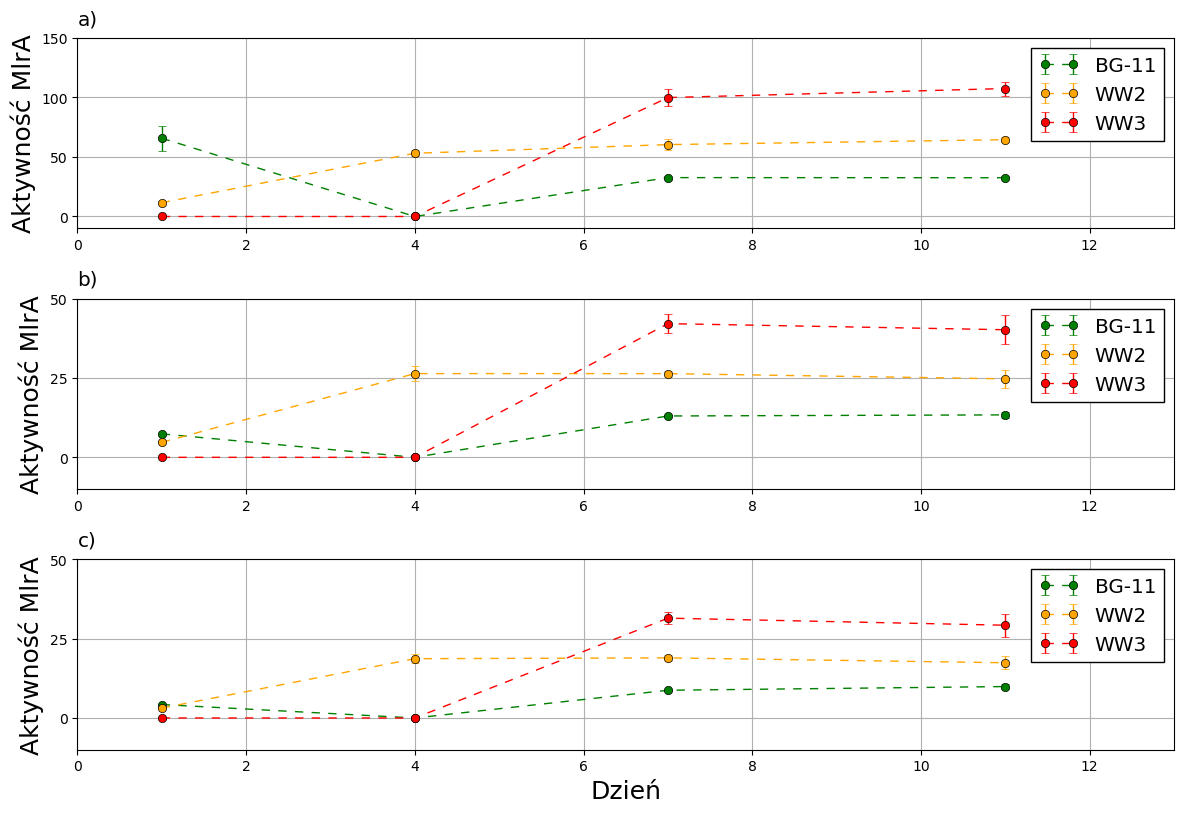
\includegraphics[width=13cm]{figures/mlra_activity}
    \caption{
        Aktywność \acrshort{mlra} w lizatach komórek
        \textit{Synechocystis sp.} PCC 6803 McCormick 7
        kultywowanych z użyciem różnych rodzajów \acrshort{ww} zmieszanych
        w proporcjach 1:1 z BG-11 jako pożywki. Słupki błędów to \acrshort{sem} (n = 3).
        Aktywność przeliczono na całkowitą zawartość białka w lizatach.
        Pomiar białka przeprowadzono w próbkach rozcieńczonych
        a) 20x; b) 50x; c) 100x.

    }
    \label{fig:3}
\end{figure}

\begin{figure}[h!]
    \centering
    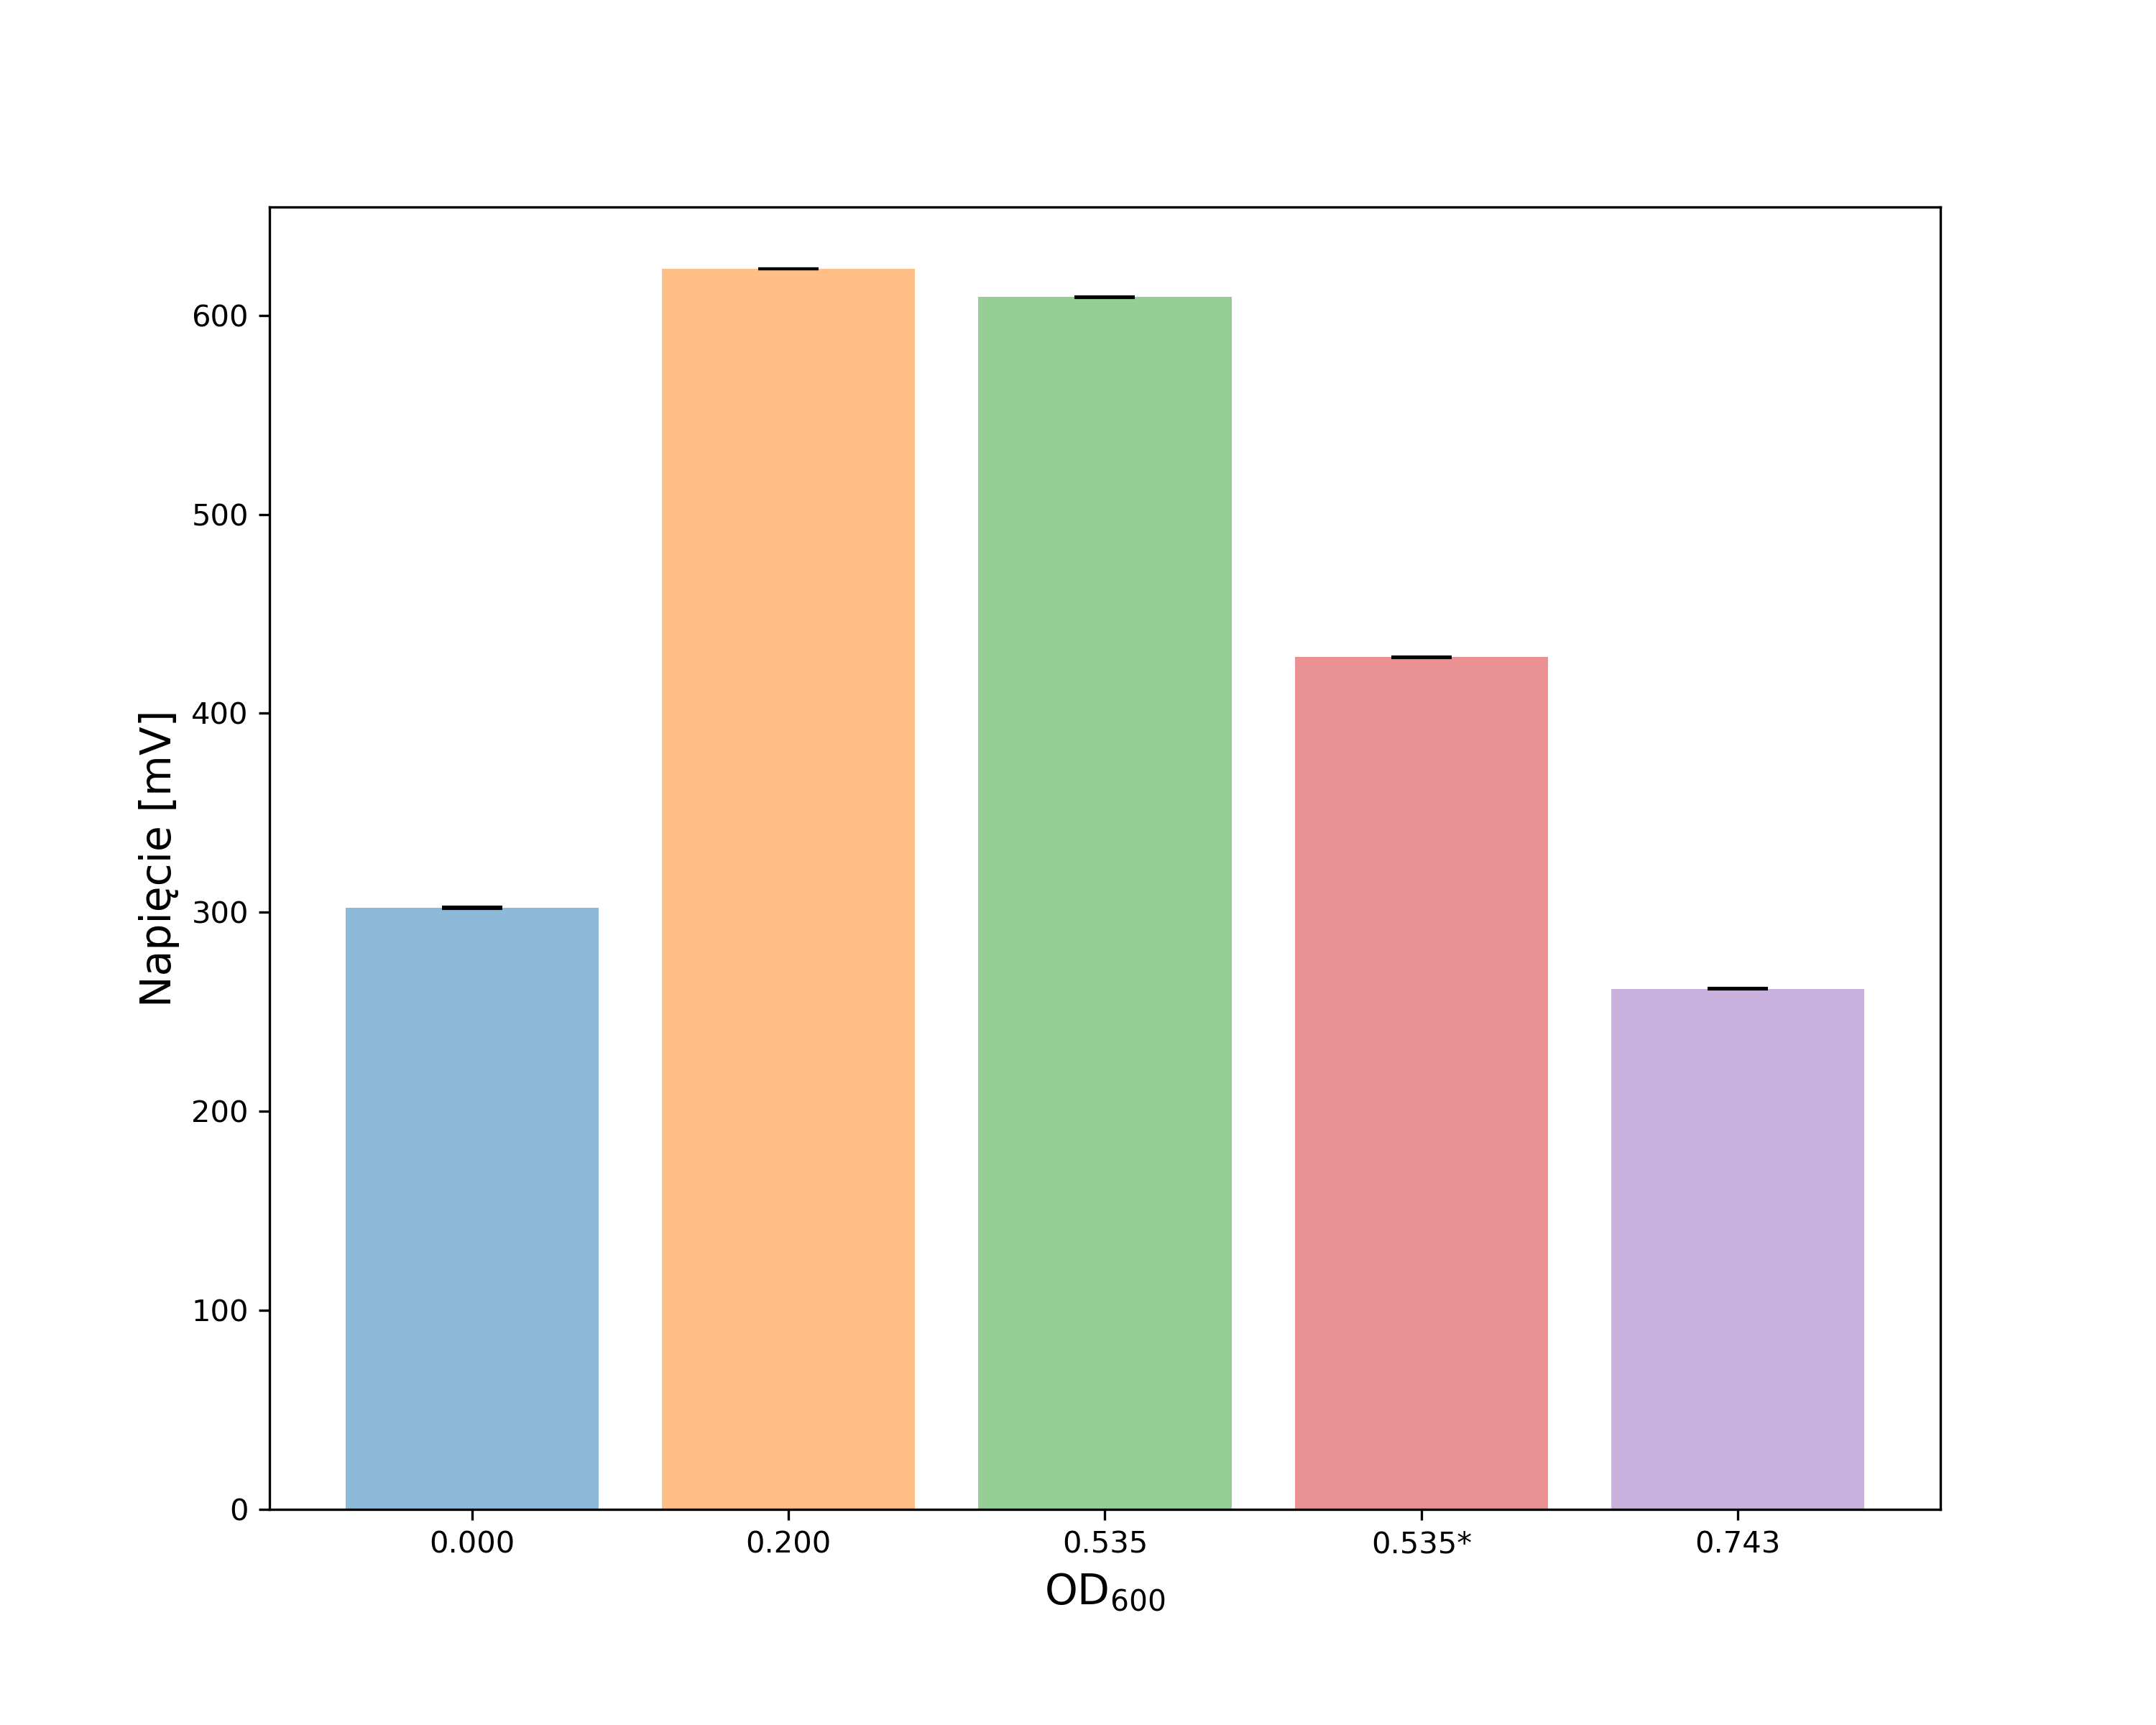
\includegraphics[width=12cm]{figures/voltage3}
    \caption{
        Uśrednione wartości napięcia w zależności od \acrshort{od}\textsubscript{600}
        hodowli \textit{R. spheroides} znajdującej się w komorze z anodą.
        *Pomiar wykonany po 24 h adaptacji mikroorganizmów do elektrody.
        Słupki błędów to \acrshort{sem} (n = 11; dla \acrshort{od}\textsubscript{600} = 0.743, n = 8).
    }
    \label{fig:4}
\end{figure}
